\documentclass[10pt,a4paper]{article}
\usepackage[textwidth=18cm,textheight=25cm]{geometry}
\usepackage[pdftex]{graphicx}
\usepackage{multirow}
% cv-custom.tex
%
% Custom macro commands and packages
% for formatting a Curriculum Vitae.
%
% Author: Matthew Earnshaw <matt@earnshaw.org.uk>
% Inspired by http://www.cv-templates.info/2009/03/professional-cv-latex/

\pagestyle{empty}

% Packages
\usepackage[usenames,dvipsnames]{color} % For custom colours
\usepackage{titlesec} % For custom section headings
\usepackage{mdwlist} % For compact lists
\usepackage[pdftex]{hyperref}
\usepackage{marvosym} % For icons

% Hyperlink colour and style
\definecolor{linkcolour}{rgb}{0,0.2,0.6}
\hypersetup{colorlinks,breaklinks, urlcolor=linkcolour, linkcolor=linkcolour}

% Custom colour
\definecolor{lgray}{gray}{0.4}

% Custom list bullet
\renewcommand{\labelitemi}{$\succ$}

% Header commands
\newcommand{\name}[1]{\LARGE\textbf{#1}}
\newcommand{\address}[1]{\color{lgray}{#1}}
\newcommand{\tel}[1]{\Large\Telefon~\small{#1}}
\newcommand{\email}[1]{\Large\Letter~\href{mailto:#1}{\small{#1}}}
\newcommand{\web}[2]{\Large\Mundus~\href{#1}{\small{#2}}}
	
% Section headings
\titleformat{\section}{\large\scshape\raggedright}{}{0em}{}[\titlerule]
\titlespacing{\section}{0pt}{0.6cm}{5pt}
% Note: Create an environment for sections ?

% Full width tables
\newenvironment{ftabular}[1]
{\begin{tabular*}{0.95\textwidth}{@{\extracolsep{\fill}}#1}}
{\end{tabular*}}

\usepackage[utf8]{inputenc}

\begin{document}
\footnotesize
\fontfamily{ptm}

\section{\sc K{\footnotesize İŞ\footnotesize İSEL} B{\footnotesize İLG\footnotesize İLER}}

\begin{tabular}{ l l l }
\vspace{0.5 mm}\\
\multirow{\fbox{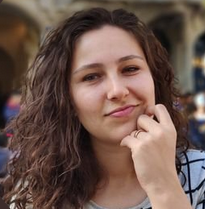
\includegraphics[height=25mm,width=20mm]{eylul.PNG}}}
& {\Huge\name{Eylül Akbaş Özköroğlu}}& Tarih: \small{16/12/2019}\\
\vspace{1 mm}\\
& \textbf{Adres :} \address{Bahçelievler Mah. İpek Sk. No:2/3 Bahçelievler/İSTANBUL} & \web{seylulgithub.io}\\
& \textbf{Doğum Tarihi :} \address{20.09.1990} & \email{akbaseylul@gmail.com}\\
& \textbf{Medeni Hal :} \address{Evli & \tel{0541 9363399}\\
& \textbf{Engellilik Durumu :} \address{Yok}  & \web{https://www.linkedin.com/in/eylul-akbas/}{linkedin}\\
\end{tabular}

\section{\sc E{\footnotesize Ğ\footnotesize İT\footnotesize İM} B{\footnotesize İLG\footnotesize İLER\footnotesize İ}}
\hspace*{1.6in}\begin{tabular}{lr}
\vspace{0.5 mm}\\
\textbf{Eğitim Seviyesi :} & Üniversite / Lisans \\
\vspace{0.5 mm}\\
\textbf{Üniversite :} & Wroclaw University of Science and Technology \\
\textbf{Fakülte/Enstitü :} &  \\
\textbf{Bölüm :} & Faculty of Computer Science and Management \\
\textbf{Öğrenim Tipi / Dili :} & Erasmus / İngilizce\\
\textbf{Not Sist. / Mez. Derecesi :} & 100 / 77.09 \\
\textbf{Başlama / Mez. Tarihi :} & Eylül  - 2012 / Haziran 2013 \\
\vspace{0.5 mm}\\
\textbf{Üniversite :} & Samsun 19 Mayıs Üniversitesi  \\
\textbf{Fakülte/Enstitü :} & Mühendislik Fakültesi \\
\textbf{Bölüm :} & Bilgisayar Mühendisliği \\
\textbf{Öğrenim Tipi / Dili :} & Örgün Öğretim / Türkçe\\
\textbf{Not Sist. / Mez. Derecesi :} & 100 / 72.04 \\
\textbf{Başlama / Mez. Tarihi :} & Eylül -2009 / Haziran -2013\\
\vspace{0.5 mm}\\
\end{tabular}

\section{\sc İ{\footnotesize Ş} D{\footnotesize ENEY\footnotesize İM\footnotesize İ}}
\begin{ftabular}
\textsc{Ekim-2013} & \textbf{Sekom A.Ş.- {\footnotesize A}nkara} \\
\vspace{0.5 mm}\\
 & \textbf{Pozisyon :} Servis Sağlayıcı -Mühendis\\
 & \textbf{İşin Tanımı :} Türkiye'nin önde gelen telekominikasyon firmalarına sağladığımız uçtan uca çözümlerde destek, kurulum, entegrasyon aşamalarında yer aldım.\\

\multicolumn{2}{c}{ } \\ % Spacer 

\textsc{Şubat-2019} & \textbf{Sekom A.Ş.- {\footnotesize İ}stanbul} \\
\vspace{0.5 mm}\\
 & \textbf{Pozisyon :} Devops & Custom Integration Engineer\\
 & \textbf{İşin Tanımı :} Devops işleri\\

\section{\sc P{\footnotesize ROGRAMLAMA} B{\footnotesize İLG\footnotesize İS\footnotesize İ}}

{\bf Çok iyi}\\
\hspace*{0.3in}\begin{tabular}{lrrrrr}
\vspace{0.5 mm}\\
  $\bullet$ C &$\bullet$ Bash &$\bullet$ Java &$\bullet$ Python &$\bullet$ Matlab &\\
\end{tabular}
\vspace{0.5 mm}\\

{\bf Güzel}\\
\hspace*{0.3in}\begin{tabular}{lrrrr}
\vspace{0.5 mm}\\
  $\bullet$ C$ \# $ &$\bullet$ Ruby &$\bullet$ Rails & $\bullet$ Php & $\bullet$ Javascript\\
\end{tabular}
\vspace{0.5 mm}\\

{\bf Orta}\\
\hspace*{0.3in}\begin{tabular}{lrrrr}
\vspace{0.5 mm}\\
  $\bullet$ Qt Creator  & & & &\\
\end{tabular}
\vspace{0.5 mm}\\

{\bf İşletim sistemleri}\\
\hspace*{0.3in}\begin{tabular}{lrrrr}
\vspace{0.5 mm}\\
  $\bullet$ GNU/Linux ( iyi ) &$\bullet$ Windows\textregistered & & &\\
\vspace{0.5 mm}\\
\end{tabular}


{\bf Belgeleme uygulamaları}\\
\hspace*{0.3in}\begin{tabular}{lrrrr}
\vspace{0.5 mm}\\
  $\bullet$ \LaTeX & & & &\\
\end{tabular}
\vspace{0.5 mm}\\


\section{\sc K{\footnotesize URS }{\footnotesize ve }S{\footnotesize EM{\footnotesize İ}NERLER}}
\begin{ftabular}{r|p{14cm}}

\textsc{30-31 mart 2013} & \textbf{JsPyConf} \\
\vspace{0.5 mm}\\
 & \textbf{Kurum Adı :}  Özyeğin Üniversitesi\\

\multicolumn{2}{c}{ } \\

\textsc{8-10 mayıs 2012} & \textbf{Yeteneğe Destek Yaratıcı Ekonomiye Destek} \\
\vspace{0.5 mm}\\
 & \textbf{Kurum Adı :}  TTNET\\

\multicolumn{2}{c}{ } \\

\textsc{25-26-27 şubat 2011} & \textbf{Bilmök 7} \\
\vspace{0.5 mm}\\
 & \textbf{Kurum Adı :}  Yeditepe Üniversitesi\\
 
\multicolumn{2}{c}{ } \\

\textsc{2-3 nisan 2010} & \textbf{Özgür Yazılım Şenliği} \\
\vspace{0.5 mm}\\
 & \textbf{Kurum Adı :}  Bilgi Üniversitesi\\

\multicolumn{2}{c}{ } \\


\end{ftabular}

\section{\sc R{\footnotesize EFERANSLAR}}

\begin{tabular}{ l l l }
\vspace{1 mm}\\
\address{Ondokuz Mayıs Üniversitesi Yrd. Doç.} & \textbf{Recai Oktaş}& \email{roktas@bil.omu.edu.tr}\\
\end{tabular}

\end{document}
